\chapter{Análisis del problema}

Los siguientes puntos tratan de plasmar los desafíos que han supuesto para mí como estudiante a la hora de comenzar el estudio y desarrollo de este proyecto.
 
\section{Red de agentes actual}

En una primera fase del proyecto, por cuestiones meramente técnicas y de aprendizaje, se procederá a simular la red de agentes que existe para el desarrollo de las prácticas de la asignatura Desarrollo Basado en Agentes. Una vez verificado todo el comportamiento del agente desarrollado, se procederá a implementar ese agente en el mismo entorno que el reso de agentes y probar así su correcto funcionamiento.\\

La arquitectura de agentes, tal y como se encontraba al momento de comienzo y con una breve explicación, es la siguiente:

\begin{itemize}
	\item \textbf{Identity Manager}: es el primer agente con el que se debe de establecer contacto en la plataforma. Encargado de verificar que somos quien decimos ser mediante el uso de nuestra \textbf{cardID}. Ningún otro agente aceptará comunicaciones de nuestro agente que no esté debidamente identificado.
	\item \textbf{World Manager}: los agentes encargados de cada práctica. Gestiona todo lo referente al \textbf{''mundo''} donde virtualmente se lleva a cabo dicha práctica.
	\item \textbf{Hackathoners}: tiene la misma funcionalidad que los agentes \textbf{World Manager}, pero estos únicamente entran en acción para los desafíos individuales.
\end{itemize}

Adicionalmente en algunas de las prácticas en grupo se implementan otros agentes que se encargarán de ciertas labores específicias, como por ejemplo, proveer al alumnado de los mapas de cada \textbf{''mundo''} para poder ubicar al dron o hacer las veces de mercado en el cual el alumnado deberá comprar los sensores que estimen oportunos para las funciones que tiene que cumplir el dron.\\

Existen también otros servicios adicionales \textit{(como el de Telegram)} que se ejecutan de manera independiente de los agentes pero que realizan labores específicas, como por ejemplo el control del progreso en la plataforma web de la asignatura o la correcta gestión y almacenamiento de la información en la base de datos.

\section{Estructura de la base de datos}

Tal y como se ha comentado en capítulos anteriores, a pesar de que el esquema actual de la base de datos, el mismo que se utilizó para el desarrollo de la asignatura y que mantendré, en consenso con el tutor de este proyecto, es mejorable en varios aspectos. No obstante, a continuación se exponen todos los aspectos relevantes con respecto a la estructura de la base de datos y sus implicaciones en el proyecto.\\

Para empezar, tenemos varias entidades independientes en la asignatura que podemos identificar de manera sencilla:

\begin{itemize}
    \item Alumnos
    \item Agentes
    \item Prácticas
    \item Problemas \textit{(asociados a cada práctica)}
    \item Insignias
    \item Analíticas de aprendizaje \textit{(en relación a LARVA)}
\end{itemize}

A medida que vayamos avanzando en las explicaciones de este apartado, surgirán de manera natural otras entidades que posteriormente serán convertidas en tablas y asociaciones entre las mismas.\\

Con respecto a los \textbf{alumnos}, surge la tabla \textbf{Users} que tiene como estructura la que se muestra en la tabla \ref{tab:usersdb}. Esta tabla es bastante intuitiva pero requirió de una columna adicional a la hora del desarrollo, una columna que almacenase el nivel de notificación \textit{(véase la tabla \ref{tab:usersdb2})} que cada usuario quisiese dentro del propio bot de Telegram. Ese nivel de notificación se podrá cambiar mediante un comando a través del mismo bot.

\begin{table}[]
\centering
\resizebox{\textwidth}{!}{%
\begin{tabular}{|l|l|c|}
\hline
\textbf{Columna} & \textbf{Descripción}                                                                                             & \textbf{Tipo} \\ \hline
userID          & Identificador único de cada usuario                                                                              & int           \\ \hline
name            & Nombre del usuario                                                                                               & string        \\ \hline
email           & Correo electrónico institucional del usuario                                                                     & string        \\ \hline
isTeacher       & \begin{tabular}[c]{@{}l@{}}Celda para especificar si el usuario es profesor\\ o no de la asignatura\end{tabular} & bool          \\ \hline
agentID         & \begin{tabular}[c]{@{}l@{}}El identificador único del agente asociado\\ a dicho alumno\end{tabular}              & int           \\ \hline
alias           & \begin{tabular}[c]{@{}l@{}}Pseudónimo bajo el que se conoce al usuario\\ en la plataforma\end{tabular}           & string        \\ \hline
chatID          & \begin{tabular}[c]{@{}l@{}}Identificador único del chat de Telegram de\\ dicho usuario\end{tabular}              & int           \\ \hline
lastUpdate      & \begin{tabular}[c]{@{}l@{}}Fecha de la última actualización del usuario\\ en la plataforma\end{tabular}          & string        \\ \hline
invitedGroup    & Grupo al que pertenece el usuario                                                                                & int           \\ \hline
\end{tabular}%
}
\caption{Estructura de la tabla \textbf{Users} en la base de datos}
\label{tab:usersdb}
\end{table}

\begin{table}[]
\centering
\resizebox{\textwidth}{!}{%
\begin{tabular}{|l|l|c|}
\hline
\textbf{Columna} & \textbf{Descripción}                                                                                             & \textbf{Tipo} \\ \hline
notificationSettings       & \begin{tabular}[c]{@{}l@{}}Nivel de notificación que el usuario\\ desea recibir\end{tabular} & string          \\ \hline
\end{tabular}%
}
\caption{Columna adicional en la tabla \textbf{Users} de la base de datos}
\label{tab:usersdb2}
\end{table}

Así pues queda definida la estructura de los usuarios del sistema. Los usuarios, a no ser que sean profesores, pertenecen también a un grupo de prácticas que se establece más adelante en el curso una vez lleguen las prácticas que requieren de grupos para ser completadas.\\

Los usuarios pertenecen a un curso concreto, modelado a través de las tablas \textbf{Courses} y \textbf{CourseRegistration} que son tablas auxiliares que mantienen un registro de los estudiantes en la asignatura por cada curso.\\

Cada curso, a su vez, tiene unas determinadas prácticas almacenadas en la tabla \textbf{Assignments}, cuya estructura se ve representada en la tabla \ref{tab:assignments}. Cada práctica puede tener unos determinados problemas que resolver. Más concretamente, como estamos en prácticas en las que se desarrolla un agente \textit{(un dron)} que se desplaza a través de un mapa concreto, estos problemas normalmente serán esos mundos o mapas que tiene que completar cada equipo con su dron correspondiente. La estructura de la tabla \textbf{Problems} se puede observar en la tabla \ref{tab:problems}.

% Please add the following required packages to your document preamble:
% \usepackage{graphicx}
\begin{table}[]
\centering
\resizebox{\textwidth}{!}{%
\begin{tabular}{|l|l|c|}
\hline
\textbf{Nombre} & \textbf{Descripción}                                                                                & \textbf{Tipo}                \\ \hline
assignmentID    & Identificador único de cada práctica                                                                & int                          \\ \hline
courseID        & Curso al que pertenece la práctica                                                                  & int                          \\ \hline
title           & Título de la práctica                                                                               & string                       \\ \hline
isActive        & Controla si la práctica está activa                                                                 & bool                         \\ \hline
singleStepAuth  & \begin{tabular}[c]{@{}l@{}}Tipo de requerimiento de\\ autenticación\end{tabular}                    & bool                         \\ \hline
releaseDate     & Fecha de comienzo                                                                                   & string                       \\ \hline
dueDate         & Fecha límite                                                                                        & string                       \\ \hline
timing          & \begin{tabular}[c]{@{}l@{}}Programación de las prácticas\\ en la asignatura\end{tabular}            & int                          \\ \hline
autoScore       & \begin{tabular}[c]{@{}l@{}}Controla si la práctica se \\ evalúa de manera automática\end{tabular}   & decimal                      \\ \hline
maxScore        & \begin{tabular}[c]{@{}l@{}}Puntuación máxima que se \\ puede obtener con esta práctica\end{tabular} & \multicolumn{1}{l|}{decimal} \\ \hline
\end{tabular}%
}
\caption{Estructura de la tabla \textbf{Problems} en la base de datos}
\label{tab:assignments}
\end{table}

% Please add the following required packages to your document preamble:
% \usepackage{graphicx}
\begin{table}[]
\centering
\resizebox{\textwidth}{!}{%
\begin{tabular}{|l|l|c|}
\hline
\textbf{Nombre}  & \textbf{Descripción}                                                                                                                            & \textbf{Tipo} \\ \hline
problemID        & Identificador único de cada problema                                                                                                            & int           \\ \hline
courseID         & Curso al que pertenece el problema                                                                                                              & int           \\ \hline
title            & Título del problema                                                                                                                             & string        \\ \hline
description      & Descripción del problema                                                                                                                        & string        \\ \hline
requireproblemID & \begin{tabular}[c]{@{}l@{}}Identificador del problema previo\\ requerido para poder completar\\ el problema actual\end{tabular}                 & int           \\ \hline
milestones       & \begin{tabular}[c]{@{}l@{}}Cadena de caracteres que representan\\ los logros de LARVA que se deben\\ de conseguir en cada problema\end{tabular} & string        \\ \hline
autoScore        & \begin{tabular}[c]{@{}l@{}}Controla el problema se \\ evalúa de manera automática\end{tabular}                                                  & int           \\ \hline
\end{tabular}%
}
\caption{Estructura de la tabla \textbf{Assignments} en la base de datos}
\label{tab:problems}
\end{table}

La última estructura que vamos a comentar es cómo se relacionan las prácticas, los problemas y las analíticas de aprendizaje con cada usuario. Esto se realiza a través de las tablas \textbf{AnalyticsReportAssignment} y \textbf{AnalyticsReportStudent} en las que, esencialmente, se almacenan los datos correspondientes de cada usuario: qué problemas ha resuelto de qué prácticas y qué metas ha conseguido de problema, y las analíticas de aprendizaje que ha conseguido el usuario. Se modelan a través de las tablas \ref{tab:arassignment} y \ref{tab:arstudent} respectivamente.\\

Para terminar este apartado, en la figura \ref{img:erbd} obtenemos el diagrama entidad-relación completo de la base de datos tal y como se encontraba al inicio del proyecto.

% Please add the following required packages to your document preamble:
% \usepackage{graphicx}
\begin{table}[]
\centering
\resizebox{\textwidth}{!}{%
\begin{tabular}{|l|l|c|}
\hline
\textbf{Nombre} & \textbf{Descripción}                                                                                                                            & \textbf{Tipo}            \\ \hline
courseID        & Curso al que pertenece el problema                                                                                                              & int                      \\ \hline
assignmentID    & \begin{tabular}[c]{@{}l@{}}Identificador único de la práctica\\ en cuestión\end{tabular}                                                        & int                      \\ \hline
whoID           & Identificador único del usuario                                                                                                                 & int                      \\ \hline
problemID       & \begin{tabular}[c]{@{}l@{}}Identificador único del problema\\ de la práctica\end{tabular}                                                       & int                      \\ \hline
milestones      & \begin{tabular}[c]{@{}l@{}}Cadena de caracteres que representan\\ los logros de LARVA que se han\\ conseguido en el problema\end{tabular}       & string                   \\ \hline

count           & Número de metas alcanzadas                                                                                                                      & int                      \\ \hline
firstsolved     & Fecha de la primera resolución                                                                                                                  & \multicolumn{1}{l|}{int} \\ \hline
latencysolved   & Tiempo que tardó en resolverse                                                                                                                  & \multicolumn{1}{l|}{int} \\ \hline
costsolved      & Costo de resolución                                                                                                                             & \multicolumn{1}{l|}{int} \\ \hline
benefitsolved   & \begin{tabular}[c]{@{}l@{}}Beneficio obtenido a través de la\\ resolución\end{tabular}                                                          & \multicolumn{1}{l|}{int} \\ \hline
firstopen       & \begin{tabular}[c]{@{}l@{}}Fecha de la primera vez que se\\ ingresó al problema\end{tabular}                                                    & \multicolumn{1}{l|}{int} \\ \hline
\end{tabular}%
}
\caption{Estructura de la tabla \textbf{AnalyticsReportAssignment} en la base de datos}
\label{tab:arassignment}
\end{table}

% Please add the following required packages to your document preamble:
% \usepackage{graphicx}
\begin{table}[]
\centering
\resizebox{\textwidth}{!}{%
\begin{tabular}{|l|l|c|}
\hline
\textbf{Nombre} & \textbf{Descripción}                                                                                                                  & \textbf{Tipo} \\ \hline
userID          & Identificador único del usuario                                                                                                       & int           \\ \hline
courseID        & Curso al que pertenece el usuario                                                                                                     & int           \\ \hline
competenceID    & \begin{tabular}[c]{@{}l@{}}Identificador único del tipo de\\ competencia\end{tabular}                                                 & string        \\ \hline
milestones      & \begin{tabular}[c]{@{}l@{}}Cadena de caracteres que representan\\ los logros de LARVA alcanzados\\ \\ en esa competencia\end{tabular} & string        \\ \hline
count           & Número de metas alcanzadas                                                                                                            & string        \\ \hline
\end{tabular}%
}
\caption{Estructura de la tabla \textbf{AnalyticsReportStudent} en la base de datos}
\label{tab:arstudent}
\end{table}

\begin{figure}[h]
\centering
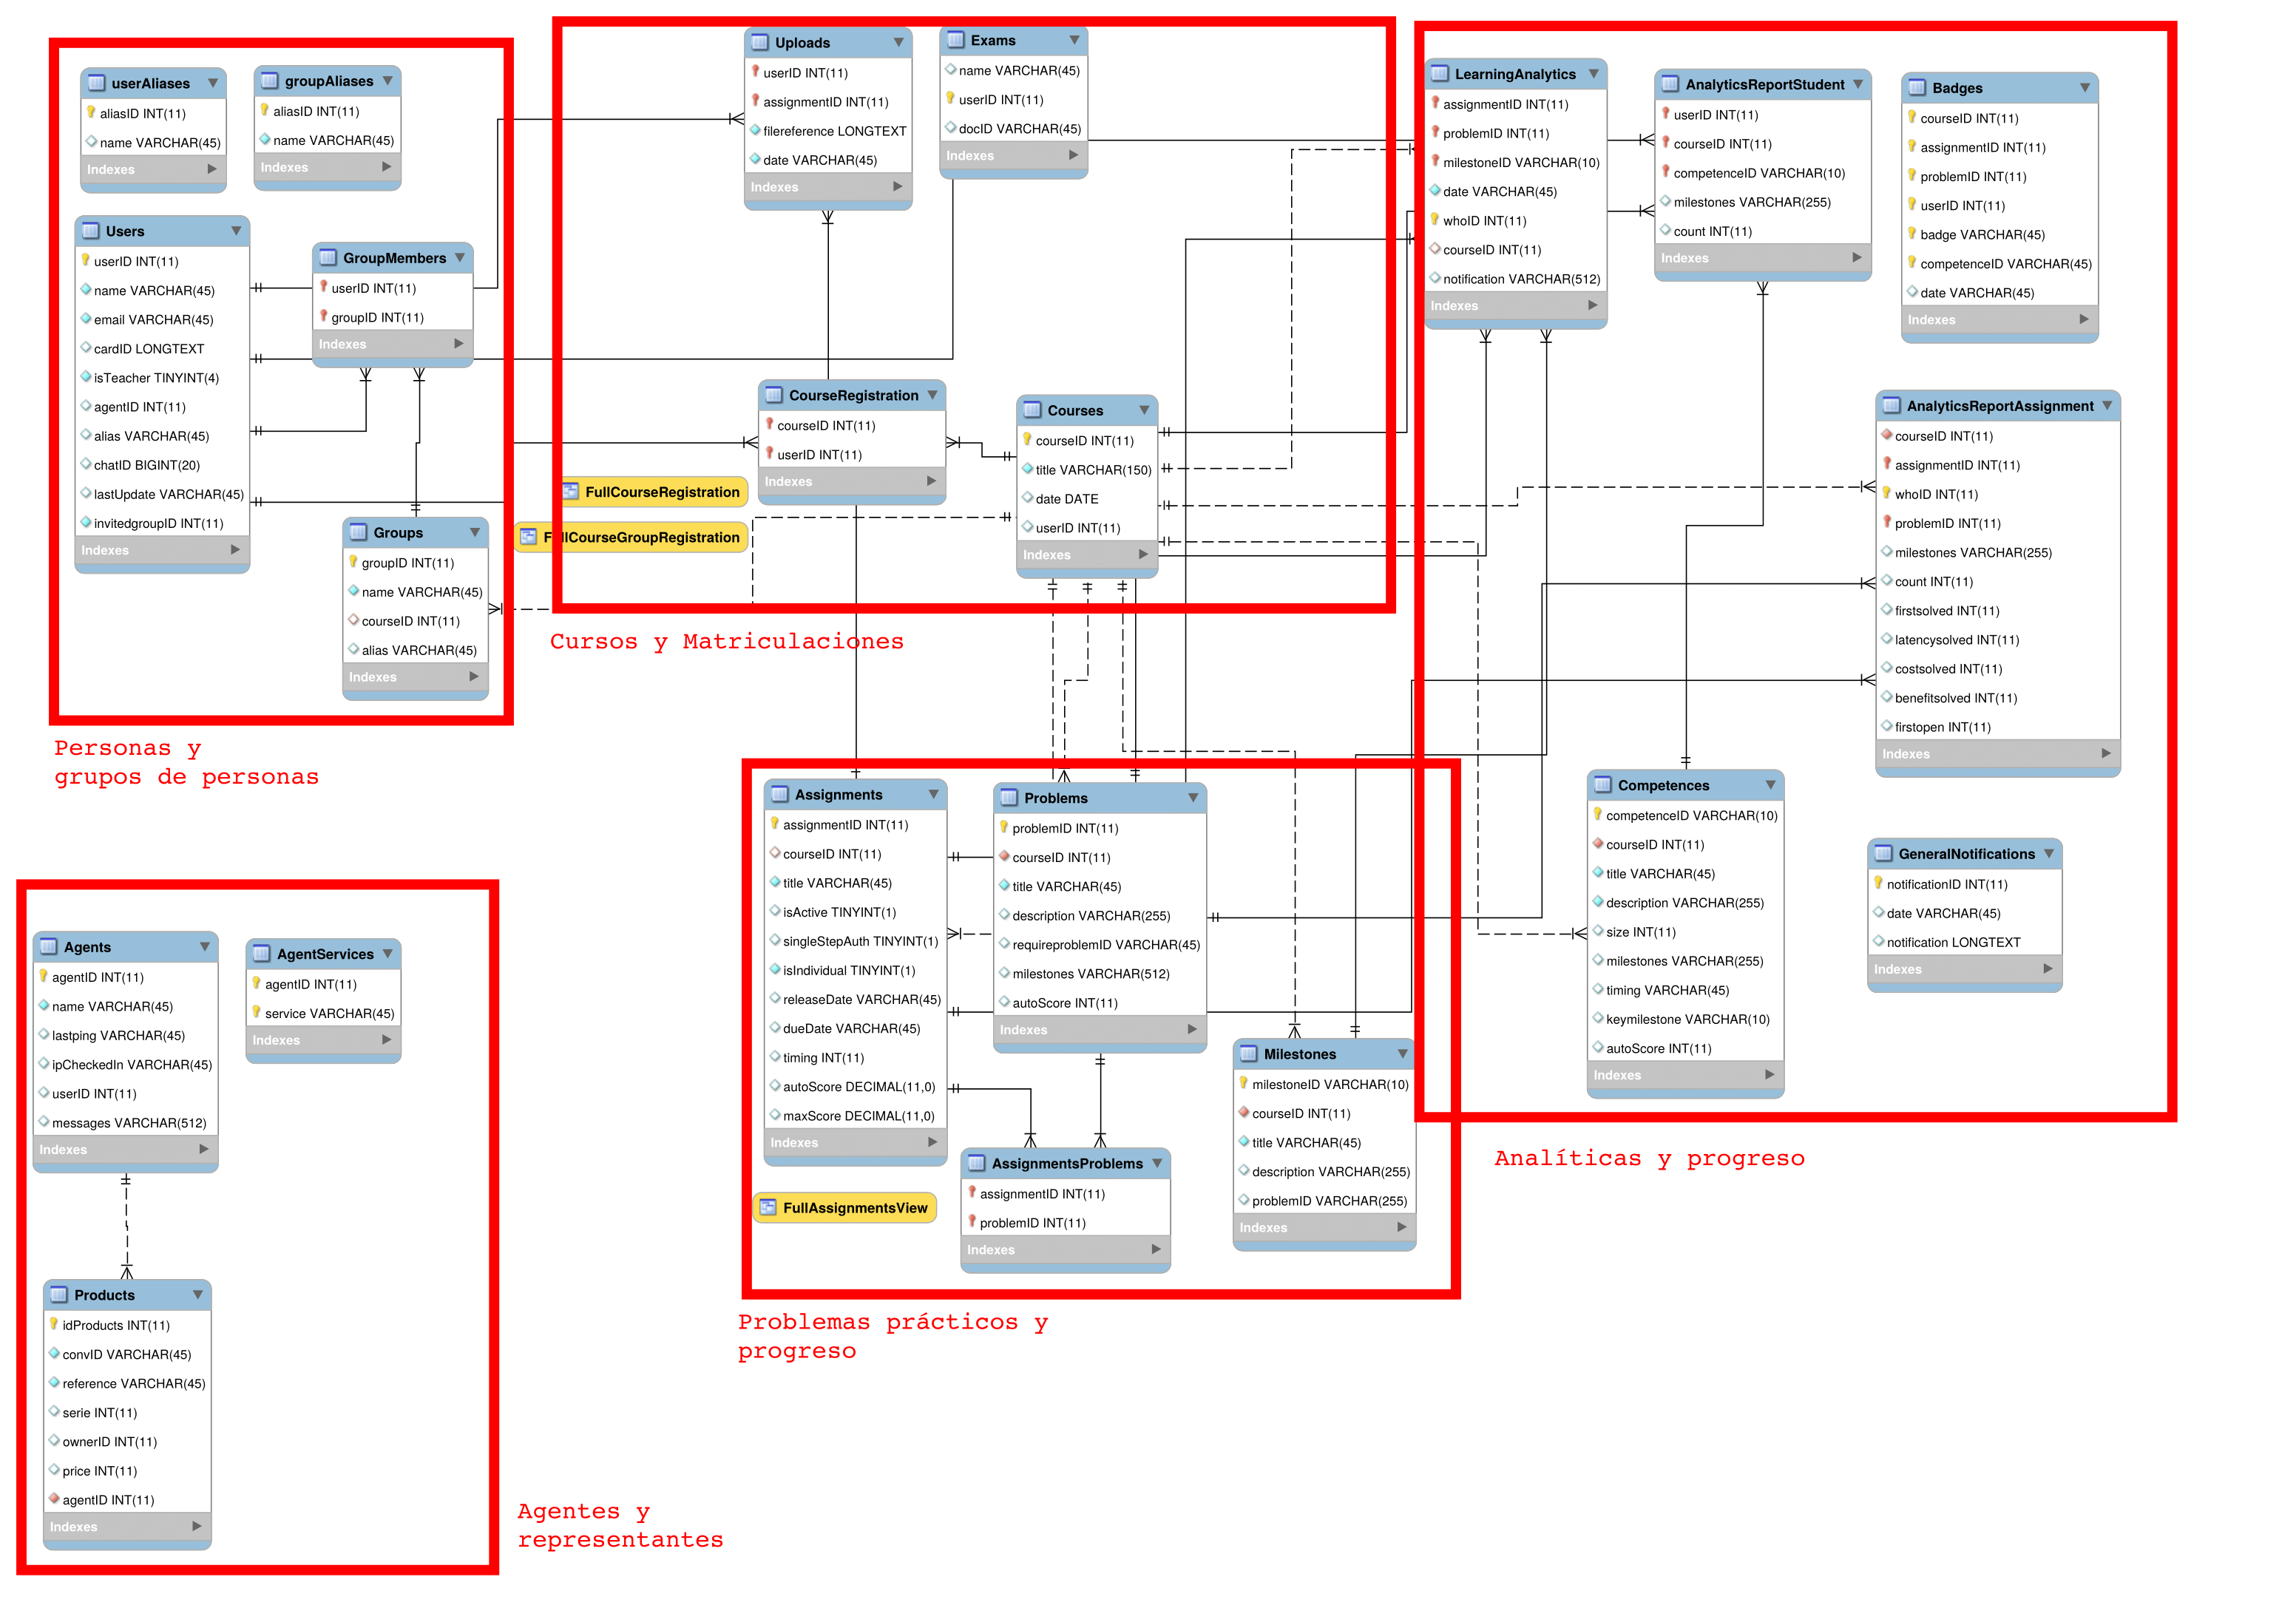
\includegraphics[width=1.35\textwidth]{logos/erbd.png}\\[1.4cm]
\caption{Diagrama entidad-relación de la base de datos del proyecto al inicio del mismo}
\label{img:erbd}
\end{figure}

\section{Bot de Telegram}

Todo lo relacionado con el comportamiento actual del bot de Telegram se gestiona a través de un servicio lanzado al mismo ecosistema de agentes de la asignatura y que se mantiene a la espera de recibir las comunicaciones de otros agentes o de los propios alumnos.\\

El funcionamiento de este bot, parte de enviar nuestra \textbf{cardID} como archivo al mismo bot. Éste hará las comprobaciones necesarias y verificará tu identidad para futuras comunicaciones con el mismo. Una vez verificada tu identidad, se establecerá una conexión con tu persona dentro de la asignatura y con tu chat único en Telegram. A través de ahí, se podrá hacer uso de los distintos comandos para obtener la retroalimentación correspondiente. Además, el bot nos informará de la ejecución de una práctica concreta: qué movimientos estamos haciendo, en qué estamos fallando, cuándo hemos completado una meta...